\documentclass{article}

\setlength{\topmargin}{-.5in}
\setlength{\oddsidemargin}{.125in}
\setlength{\textwidth}{6.25in}

% page numbering style
\usepackage{fancyhdr}
\pagestyle{fancy}
\renewcommand{\headrulewidth}{0pt}
\fancyhf{}
\fancyfoot[R]{\thepage}
\fancypagestyle{plain}{%
    \renewcommand{\headrulewidth}{0pt}%
    \fancyhf{}%
    \fancyfoot[R]{\thepage}%
}

\usepackage{float}

\usepackage{Sweave}
\begin{document}
\Sconcordance{concordance:report.tex:report.Rnw:%
1 20 1 1 0 2 1 1 12 1 4 1 25 23 1 1 19 2 1 2 2 342 1 1 43 2 1 2 2 2 1 1 %
34 1 22 1 3 4 0 1 2 1 1}





\title{Mathematics Developers Survey 2016}
\author{Nejc Ileni\v{c}}
\date{}
\maketitle

\section{Introduction}
Anonymised responses from Stack Overflow Annual Developer Survey are published each year along the results to encourage their further analysis. Being curious about where in the world an aspiring data scientist should start his/her career, I have decided to use the available data in an attempt to answer this question and to learn more about people identifying themselves as mathematics developers.

The survey consisted mostly of demographic questions and questions regarding professional work and technology. Some specific questions that we will seek answers to are \textit{In which countries are mathematics developers most satisfied with their jobs?}, \textit{In which countries do mathematics developers make the most money?}, \textit{How is compensation related to the level of satisfaction}? and alike.

\vspace{2mm}

An important thing to note when interpreting the results however is that this data may not be a represantative sample from the population of mathematics developers. One should keep in mind that these are developers who were aware of the survey and were willing to answer the questions.

\section{Data Preparation}
The dataset was constructed from survey that took place from January 7 to January 25, 2016, with responses originating from Stack Overflow, Stack Exchange technical sites, Facebook and Twitter. Raw data consists of 56030 samples and 66 features, all of which are optional.

In order to obtain an adequately sizable sample, I have decided to include all respondents that belong to the occupation group of mathematics developers, which includes data scientists, machine learning developers and developers with statistics and mathematics backgrounds. After filtering out other occupations and responses with unknown countries we are left with 2132 samples.

\vspace{2mm}

Number of mathematics developers per country can be seen in Figure \ref{fig_0}. Minimum number of 40 respondents is required to take the country into account and all others are placed into a single group called \textit{Other}. Note that selected countries and number of people may be different when doing inference of specific features due to missing values (i.e. optional answers in the survey). Majority of respondents are from United States, followed by a combination of countries with less than 40 developers, United Kingdom, Germany and India.


\begin{figure}[H]
\centering
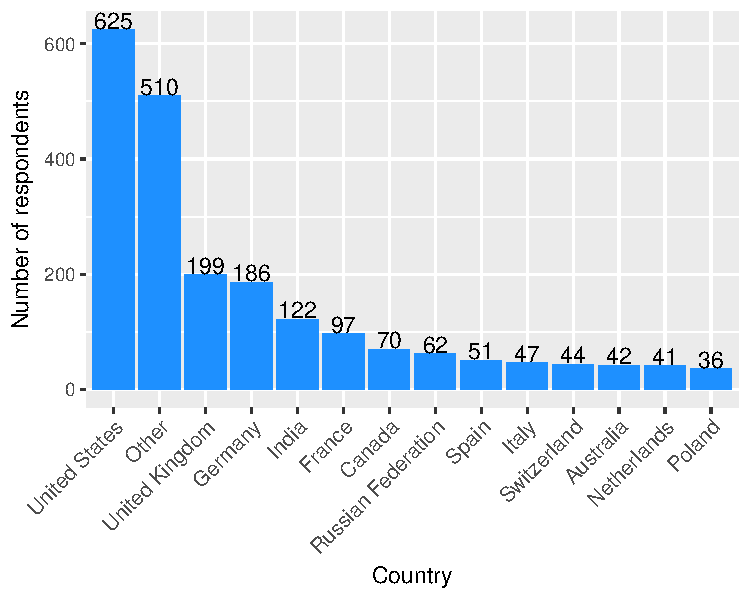
\includegraphics{report-005}
\caption{Number of mathematics developers per country.}\label{fig_0}
\end{figure}

\section{Exploratory Analysis}
todo

\subsection{Job Satisfaction}
% todo
% 
% <<echo=FALSE>>=
% # JOB SATISFACTION COMPARISON: data preparation
% params = c('theta[1]', 'theta[2]', 'theta[3]', 'theta[4]', 'theta[5]')
% params.labels = c(
%   'I hate my job',
%   'I\'m somewhat dissatisfied with my job',
%   'I\'m neither satisfied nor dissatisfied',
%   'I\'m somewhat satisfied with my job',
%   'I love my job'
% )
% params.satisfied = 5
% params.unsatisfied = c(1, 2, 3, 4)
% 
% data.satisfaction = GetNonNaData('job_satisfaction')
% data.satisfaction$country = droplevels(data.satisfaction$country)
% data.satisfaction = data.satisfaction[data.satisfaction$job_satisfaction != 'I don\'t have a job',]
% data.satisfaction$job_satisfaction = droplevels(data.satisfaction$job_satisfaction)
% 
% # reorder factor levels
% reordered.levels = levels(data.satisfaction$job_satisfaction)[c(1, 4, 3, 5, 2)]
% data.satisfaction$job_satisfaction = factor(data.satisfaction$job_satisfaction, reordered.levels)
% @
% 
% <<echo=FALSE>>=
% # JOB SATISFACTION COMPARISON: stan data preparation
% countries = unique(data.satisfaction$country)
% stan.data = list()
% 
% for (country in countries) {
%   y = as.numeric(data.satisfaction[data.satisfaction$country == country, 'job_satisfaction'])
%   stan.data[[country]] = list(
%     n = length(y),
%     k = length(params),
%     y = y,
%     a = c(1, 1, 1, 1, 1)
%   )
% }
% @
% 
% <<computation,results=hide,echo=FALSE>>=
% # JOB SATISFACTION COMPARISON: model fitting and diagnostic plots saving
% stan.fits = list()
% 
% for (country in countries) {
%   # fit a model
%   stan.fits[[country]] = stan(
%     file = '../models/multinomial_dirichlet.stan',
%     data = stan.data[[country]],
%     iter = 1000,
%     warmup = 300,
%     chains = 1
%   )
% 
%   trace.plot = traceplot(stan.fits[[country]], pars = params)
%   ggsave(
%     paste('../plots/job_satisfaction_comparison_traceplot_', tolower(country), '.png', sep = ''),
%     trace.plot
%   )
% 
%   summ = summary(stan.fits[[country]], pars = params)$summary
%   write.table(
%     summ,
%     paste('../mcmc_summaries/job_satisfaction_comparison_summary_', tolower(country), '.txt', sep = '')
%   )
% }
% @
% 
% <<echo=FALSE>>=
% # JOB SATISFACTION COMPARISON: posterior predictive check (satisfied - not satisfied log odds ratio)
% empirical.logodds = data.frame()
% posterior.logodds = data.frame()
% 
% for (country in countries) {
%   observed.dataset = stan.data[[country]]$y
%   n = stan.data[[country]]$n
%   pred.datasets = extract(stan.fits[[country]], pars = 'y_datasets')$y_datasets
% 
%   # empirical log odds
%   num.satisfied = length(Filter(function(x) x == params.satisfied, observed.dataset))
%   num.unsatisfied = length(Filter(function(x) x %in% params.unsatisfied, observed.dataset))
%   df = data.frame(lo = log(num.satisfied / num.unsatisfied), n = n, country = country)
%   empirical.logodds = rbind(empirical.logodds, df)
% 
%   # replicated log odds
%   num.satisfied = pred.datasets[, params.satisfied]
%   num.unsatisfied = rowSums(pred.datasets[, params.unsatisfied])
%   df = data.frame(lo = log(num.satisfied / num.unsatisfied), country = country)
%   posterior.logodds = rbind(posterior.logodds, df)
% }
% 
% posterior.check.plot = ggplot(posterior.logodds, aes(x = lo)) +
%   geom_histogram(binwidth = .2, fill = 'dodgerblue') +
%   geom_vline(data = empirical.logodds, aes(xintercept = lo), colour = 'red') +
%   facet_wrap(~country) +
%   labs(x = 'posterior predictive log odds', y = 'count')
% 
% ggsave(
%   paste('../plots/job_satisfaction_comparison_posterior_check.png'),
%   posterior.check.plot
% )
% @
% 
% \begin{figure}[H]
% \centering
% <<fig=True,width=5,height=4,echo=FALSE>>=
% posterior.check.plot
% @
% \caption{todo.}\label{fig_1}
% \end{figure}
% 
% <<echo=FALSE>>=
% # JOB SATISFACTION COMPARISON: posterior parameters
% errorbars = data.frame()
% 
% for (country in countries) {
%   summ = summary(stan.fits[[country]], pars = params[5], probs = c(0.05, 0.95))$summary
%   df = data.frame(
%     mean = summ[, c('mean')],
%     ci.low = summ[, c('5%')],
%     ci.up = summ[, c('95%')]
%   )
%   df$country = country
% 
%   errorbars = rbind(errorbars, df)
% }
% 
% errorbars.plot = ggplot(errorbars) +
%   geom_errorbarh(
%     aes(x = ci.up, xmin = ci.low, xmax = ci.up, y = country, color = country),
%     size = 1.5,
%     height = .5
%   ) +
%   geom_point(aes(x = mean, y = country), fill = 'white', size = 2, shape = 21) +
%   theme(legend.position = 'none')
% 
% ggsave(
%   paste('../plots/job_satisfaction_comparison_posterior_parameters.png'),
%   errorbars.plot
% )
% @
% 
% \begin{figure}[H]
% \centering
% <<fig=True,width=5,height=4,echo=FALSE>>=
% errorbars.plot
% @
% \caption{todo.}\label{fig_2}
% \end{figure}
% 
% <<echo=FALSE>>=
% # JOB SATISFACTION EFFECTS: data preparation
% 
% cols = c(
%   'age_midpoint', 'gender', 'salary_midpoint', 'remote', 'job_satisfaction',
%   'big_mac_index', 'unit_testing', 'commit_frequency', 'company_size_range',
%   'education'
% )
% relationships.data = na.omit(data.cleaned[, cols])
% 
% relationships.data$purchasing_power = relationships.data$salary_midpoint / relationships.data$big_mac_index
% relationships.data = relationships.data[, !(names(relationships.data) %in% c('salary_midpoint', 'big_mac_index'))]
% 
% # job_satisfaction
% # 'I hate my job',
% # 'I\'m somewhat dissatisfied with my job',
% # 'I\'m neither satisfied nor dissatisfied',
% # 'I\'m somewhat satisfied with my job',
% # 'I love my job'
% relationships.data = relationships.data[relationships.data$job_satisfaction != 'I don\'t have a job',]
% relationships.data$job_satisfaction = droplevels(relationships.data$job_satisfaction)
% reordered.levels = levels(relationships.data$job_satisfaction)[c(1, 4, 3, 5, 2)]
% relationships.data$job_satisfaction = factor(relationships.data$job_satisfaction, reordered.levels)
% relationships.data$job_satisfaction = as.numeric(relationships.data$job_satisfaction)
% 
% # gender
% # 'Female'
% # 'Male'
% relationships.data$gender = as.numeric(relationships.data$gender)
% relationships.data$gender_male = relationships.data$gender - 1
% relationships.data = relationships.data[, names(relationships.data) != 'gender']
% 
% # unit_testing
% # 'No'
% # 'Yes'
% relationships.data = relationships.data[relationships.data$unit_testing != 'I don\'t know',]
% relationships.data$unit_testing = droplevels(relationships.data$unit_testing)
% relationships.data$unit_testing = as.numeric(relationships.data$unit_testing)
% relationships.data$unit_testing = relationships.data$unit_testing - 1
% 
% # remote
% # 'Never'
% # 'I rarely work remotely'
% # 'Part-time remote'
% # 'Full-time remote'
% reordered.levels = levels(relationships.data$remote)[c(3, 2, 4, 1)]
% relationships.data$remote = factor(relationships.data$remote, reordered.levels)
% relationships.data$remote = as.numeric(relationships.data$remote)
% # 'No'
% # 'Yes'
% relationships.data$remote = as.numeric(relationships.data$remote > 2)
% # relationships.data = DummyEncode(relationships.data, 'remote')
% 
% # commit_frequency
% # 'I never check-in or commit code'
% # 'A few times a month'
% # 'A couple times a week'
% # 'Once a day'
% # 'Multiple times a day'
% omit = 'I don\'t \"check-in or commit code\", but I do put code into production somewhat frequently'
% relationships.data = relationships.data[relationships.data$commit_frequency != omit,]
% relationships.data$commit_frequency = droplevels(relationships.data$commit_frequency)
% reordered.levels = levels(relationships.data$commit_frequency)[c(3, 2, 1, 5, 4)]
% relationships.data$commit_frequency = factor(relationships.data$commit_frequency, reordered.levels)
% relationships.data$commit_frequency = as.numeric(relationships.data$commit_frequency)
% # commit at least once a day
% # 'No'
% # 'Yes'
% relationships.data$commit_once_a_day = as.numeric(relationships.data$commit_frequency > 3)
% relationships.data = relationships.data[, names(relationships.data) != 'commit_frequency']
% 
% # company_size_range
% relationships.data = relationships.data[relationships.data$company_size_range != 'I am not sure',]
% relationships.data$company_size_range = droplevels(relationships.data$company_size_range)
% reordered.levels = levels(relationships.data$company_size_range)[c(10, 1, 7, 3, 6, 5, 9, 2, 8, 4)]
% relationships.data$company_size_range = factor(relationships.data$company_size_range, reordered.levels)
% relationships.data$company_size_range = as.numeric(relationships.data$company_size_range)
% # big company
% # 'No'
% # 'Yes'
% relationships.data$big_company = as.numeric(relationships.data$company_size_range > 5)
% relationships.data = relationships.data[, names(relationships.data) != 'company_size_range']
% 
% # phd
% relationships.data$phd = as.numeric(Map(function(x) grepl('PhD', x), relationships.data$education))
% relationships.data = relationships.data[, names(relationships.data) != 'education']
% @
% 
% <<echo=FALSE>>=
% # JOB SATISFACTION EFFECTS: stan data preparation
% x = relationships.data[, names(relationships.data) != 'job_satisfaction']
% 
% # center, scale
% x$purchasing_power = (x$purchasing_power - mean(x$purchasing_power)) / sd(x$purchasing_power)
% x$age_midpoint = (x$age_midpoint - mean(x$age_midpoint)) / sd(x$age_midpoint)
% 
% y = relationships.data$job_satisfaction
% 
% k = length(unique(y))
% stan.data = list(
%   n = nrow(x),
%   k = k,
%   d = ncol(x),
%   y = y,
%   x = x
% )
% @
% 
% <<computation,results=hide,echo=FALSE>>=
% # JOB SATISFACTION EFFECTS: model fitting and diagnostic plots saving
% params = c(
%   paste('beta[', 1:ncol(x), ']', sep = ''),
%   paste('threshold[', seq(1, k - 1, 1), ']', sep = '')
% )
% 
% stan.fit = stan(
%   file = '../models/ordinal_logistic_regression.stan',
%   data = stan.data,
%   iter = 1000,
%   warmup = 300,
%   chains = 1
% )
% 
% # save a traceplot
% trace.plot = traceplot(stan.fit, pars = params)
% ggsave('../plots/job_satisfaction_effects_traceplot.png', trace.plot)
% 
% summ = summary(stan.fit, pars = params)$summary
% write.table(summ, file = '../mcmc_summaries/job_satisfaction_effects_summary.txt')
% @
% 
% <<echo=FALSE>>=
% # JOB SATISFACTION EFFECTS: regressors correlation
% corr = round(cor(cbind(x, y)), 2)
% corr.plot = ggcorrplot(
%   corr,
%   lab = TRUE,
%   lab_size = 2.5,
%   outline.col = "white",
%   colors = c('#6D9EC1', 'white', '#E46726'),
%   legend.title = 'Correlation',
%   tl.cex = 8
% )
% ggsave('../plots/job_satisfaction_effects_regressors_correlation.png', corr.plot)
% @
% 
% \begin{figure}[H]
% \centering
% <<fig=True,width=5,height=4,echo=FALSE>>=
% corr.plot
% @
% \caption{todo.}\label{fig_3}
% \end{figure}
% 
% <<echo=FALSE>>=
% # JOB SATISFACTION EFFECTS: posterior parameters
% posterior.params = as.data.frame(stan.fit, pars = params[1:ncol(x)])
% names(posterior.params) = names(x)
% 
% posterior.params.plot = ggplot(stack(posterior.params)) +
%   geom_boxplot(aes(x = factor(ind, levels = names(posterior.params)), y = values, fill = ind), notch = TRUE) +
%   theme(
%     legend.position = 'none',
%     axis.text.x = element_text(
%       angle = 45,
%       hjust = 1,
%       vjust = 1
%     )
%   ) +
%   labs(x = 'todo', y = 'todo')
% 
% ggsave('../plots/job_satisfaction_effects_posterior_parameters.png', posterior.params.plot)
% @
% 
% \begin{figure}[H]
% \centering
% <<fig=True,width=5,height=4,echo=FALSE>>=
% posterior.params.plot
% @
% \caption{todo.}\label{fig_4}
% \end{figure}

\subsection{Purchasing Power}
todo


\begin{figure}[H]
\centering
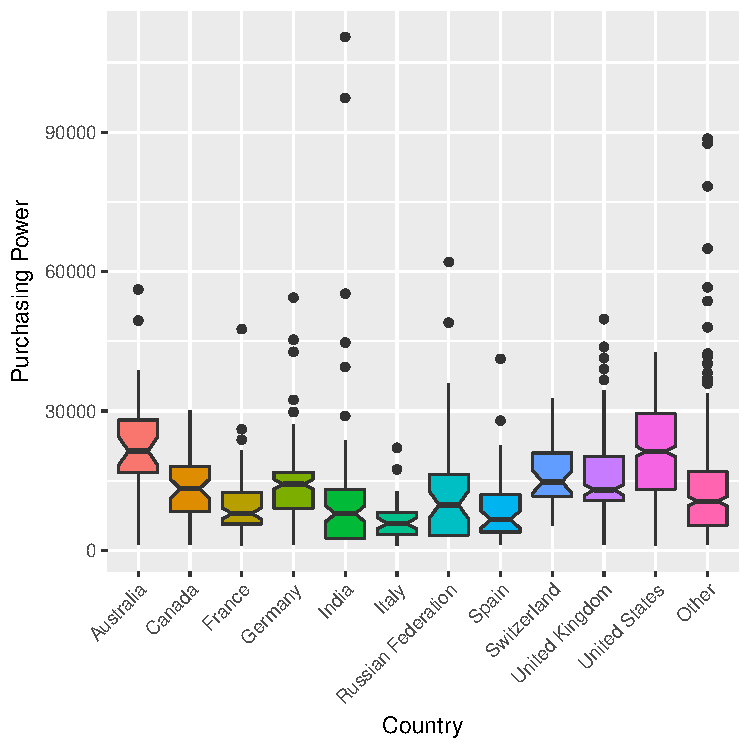
\includegraphics{report-007}
\caption{todo.}\label{fig_5}
\end{figure}



\begin{Schunk}
\begin{Soutput}
[1] "todo"
\end{Soutput}
\end{Schunk}

\end{document}
